\documentclass{standalone}
\usepackage{ tikz }
\usepackage{ xparse }
\usepackage{ ../../../macros }

\begin{document}
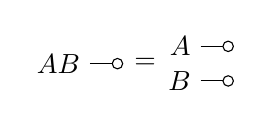
\begin{tikzpicture}[yscale=-1,x=1em,y=1.25em]
    \node [anchor=east] at (-1,0) {$A \tensor B$};
    \draw [] (-1,0) -- (0,0);
    \node [draw, circle, fill=white, scale=0.4] at (0,0) {};

    \node at (1,0) {$=$};

    \node [anchor=east] at (3,-0.5) {$A$};
    \node [anchor=east] at (3,0.5) {$B$};

    \draw (3,-0.5) -- (4,-0.5);
    \draw (3,0.5) -- (4,0.5);

    \node [draw, circle, fill=white, scale=0.4] at (4,-0.5) {};
    \node [draw, circle, fill=white, scale=0.4] at (4,0.5) {};

\end{tikzpicture}
\end{document}